\chapter{Implementacija i korisničko sučelje}
		
		
		\section{Korištene tehnologije i alati}
		
			Komunikacija u timu ostvarena je kombinacijom \textbf{Atlassin Jira}, \textbf{Atlassin Confluence} i \textbf{WhatsApp}. Za upravljanje kodom korišten je sustav \textbf{Git} i web platforma \textbf{GitHub} za pregled udaljenog repozitorija i bolje snalaženje u projektu.
			Kao razvojno okruženje korišteni su \textbf{Microsoft Visual Studio Code} i \textbf{JetBrains PyCharm}. Microsoft Visual Studio Code pruža integrirano razvojno okruženje (IDE) koje podržava različite programske jezike, uključujući C++, Python i mnoge druge. Ovo okruženje dolazi s alatima za uređivanje koda, debugiranje i upravljanje datotekama i kontejnerima.
			S druge strane, \textbf{JetBrains PyCharm} je posebno usmjeren na podršku Python razvoju. Ovaj IDE pruža bogat skup značajki, uključujući pametno završavanje koda, analizu koda, integrirano upravljanje verzijama, i podršku za virtualno okruženje. Korištenjem ova dva razvojna okruženja, tim je imao pristup snažnim alatima za učinkovit i produktivan razvoj softvera.
			Aplikacija je napisana koristeći radni okvir \textbf{FastApi} koji se koristi za izradu REST API-ja u pythonu. Za izradu \textit{frontenda} koristili smo \textbf{React} i \textbf{TypeScript}. Prednost \textbf{TypeScripta} nad običnim \textbf{Javascriptom} je u njegovoj mogućnosti definiranja tipa varijabli i posljedično tome, lakšem rukovanju greškama i boljom kontrolom varijabli.
			Za izradu kontejnera je korišten \textbf{Docker}, a sve je stavljeno na poslužitelja u oblaku na \textbf{Microsoft Azure}.
			
			
			
			\eject 
		
	
		\section{Ispitivanje programskog rješenja}
			
			\textbf{\textit{dio 2. revizije}}\\
			
			 \textit{U ovom poglavlju je potrebno opisati provedbu ispitivanja implementiranih funkcionalnosti na razini komponenti i na razini cijelog sustava s prikazom odabranih ispitnih slučajeva. Studenti trebaju ispitati temeljnu funkcionalnost i rubne uvjete.}
	
			
			\subsection{Ispitivanje komponenti}
			\textit{Potrebno je provesti ispitivanje jedinica (engl. unit testing) nad razredima koji implementiraju temeljne funkcionalnosti. Razraditi \textbf{minimalno 6 ispitnih slučajeva} u kojima će se ispitati redovni slučajevi, rubni uvjeti te izazivanje pogreške (engl. exception throwing). Poželjno je stvoriti i ispitni slučaj koji koristi funkcionalnosti koje nisu implementirane. Potrebno je priložiti izvorni kôd svih ispitnih slučajeva te prikaz rezultata izvođenja ispita u razvojnom okruženju (prolaz/pad ispita). }
			
			
			
			\subsection{Ispitivanje sustava}
			
			 \textit{Potrebno je provesti i opisati ispitivanje sustava koristeći radni okvir Selenium\footnote{\url{https://www.seleniumhq.org/}}. Razraditi \textbf{minimalno 4 ispitna slučaja} u kojima će se ispitati redovni slučajevi, rubni uvjeti te poziv funkcionalnosti koja nije implementirana/izaziva pogrešku kako bi se vidjelo na koji način sustav reagira kada nešto nije u potpunosti ostvareno. Ispitni slučaj se treba sastojati od ulaza (npr. korisničko ime i lozinka), očekivanog izlaza ili rezultata, koraka ispitivanja i dobivenog izlaza ili rezultata.\\ }
			 
			 \textit{Izradu ispitnih slučajeva pomoću radnog okvira Selenium moguće je provesti pomoću jednog od sljedeća dva alata:}
			 \begin{itemize}
			 	\item \textit{dodatak za preglednik \textbf{Selenium IDE} - snimanje korisnikovih akcija radi automatskog ponavljanja ispita	}
			 	\item \textit{\textbf{Selenium WebDriver} - podrška za pisanje ispita u jezicima Java, C\#, PHP koristeći posebno programsko sučelje.}
			 \end{itemize}
		 	\textit{Detalji o korištenju alata Selenium bit će prikazani na posebnom predavanju tijekom semestra.}
			
			\eject 
		
		
		\section{Dijagram razmještaja}

			 Dijagrami razmještaja opisuju topologiju sklopovlja i programsku potporu koja se koristi u implementaciji sustava u njegovom radnom okruženju.
			 Na azure app service-u nalaze se API sa evaluatorom rješenja, poslužitelj baze podataka (azure sql database) te third party servis za kompajliranje koda.
			 Klijenti koriste web preglednik za pristup web aplikaciji. Sustav je baziran na REST API arhitekturi, a komunikacija između klijenta i poslužitelja odvija se preko HTTP veze.

			 
			
			\begin{figure}[H]
				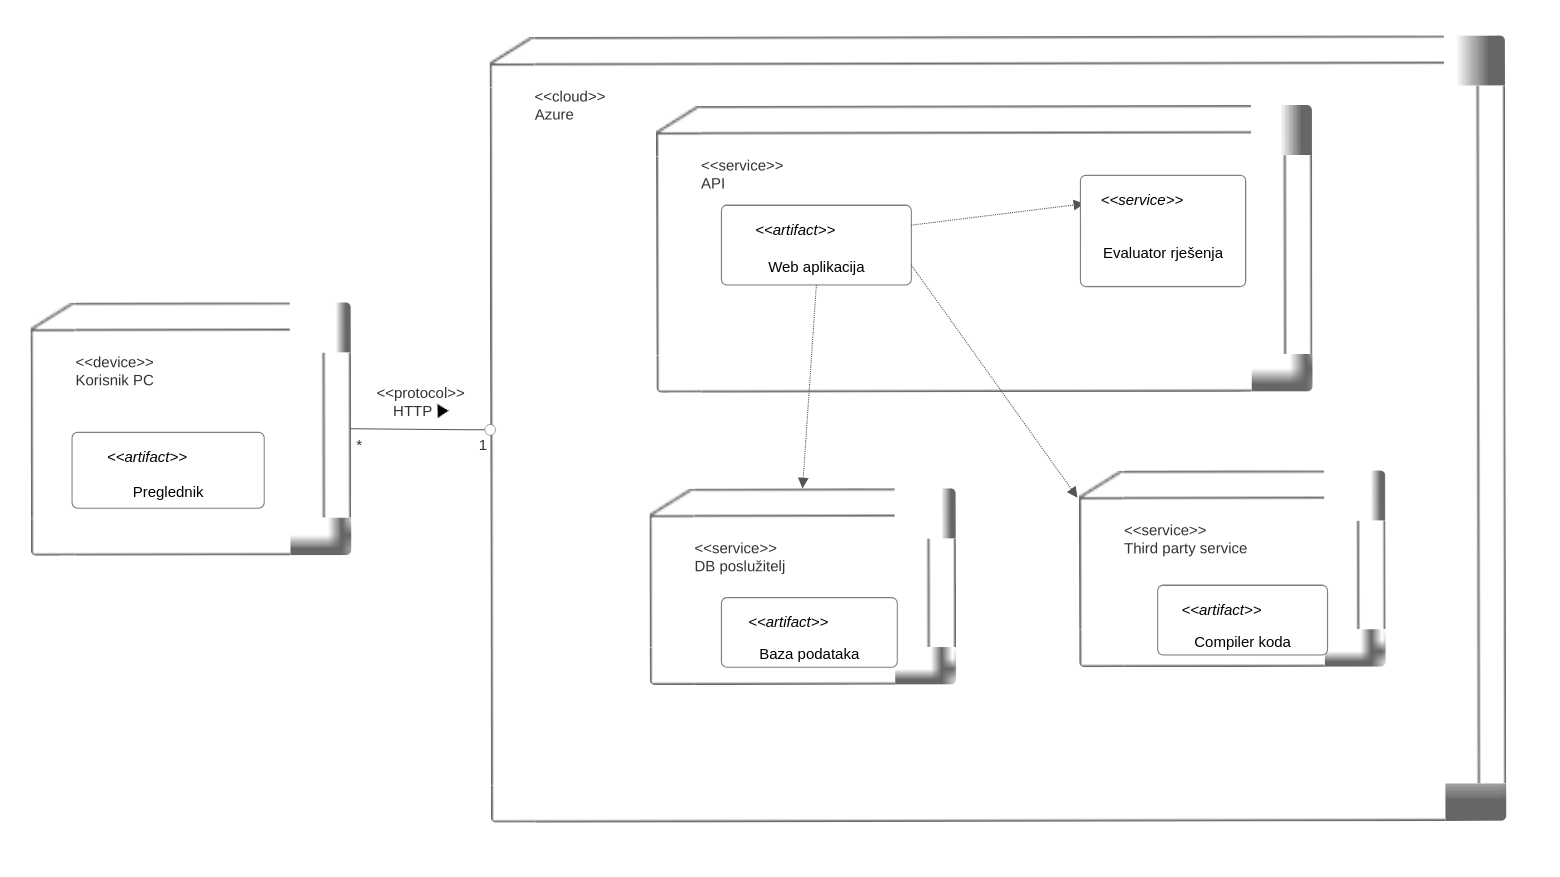
\includegraphics[width=\linewidth]{slike/dijagram_razmjestaja.png} 
				\centering
				\caption{Dijagram razmještaja}
				\label{fig:razmjestaj}
			\end{figure}
			\eject 
		
		\section{Upute za puštanje u pogon}
		
			\textbf{Pokretanje backend-a i baze podataka}\\
			
				\noindent Potrebno je preuzeti i instalirati aplikaciju \href{https://www.docker.com/products/docker-desktop/}{Docker Desktop} uz pomoć koje se pokreću container-i za backend i bazu podataka. Nakon preuzimanja aplikacije moramo se u terminalu navigirati do direktorija \textit{bytepit-root} unutar kojeg se nalazi docker-compose datoteka koja sadrži informacije za pokretanje. Pri prvom pokretanju potrebno je nekoliko minuta za podizanje.\\
				Unutar terminala koristimo naredbu: \textbf{docker-compose up --build}
				\begin{figure}[H]
					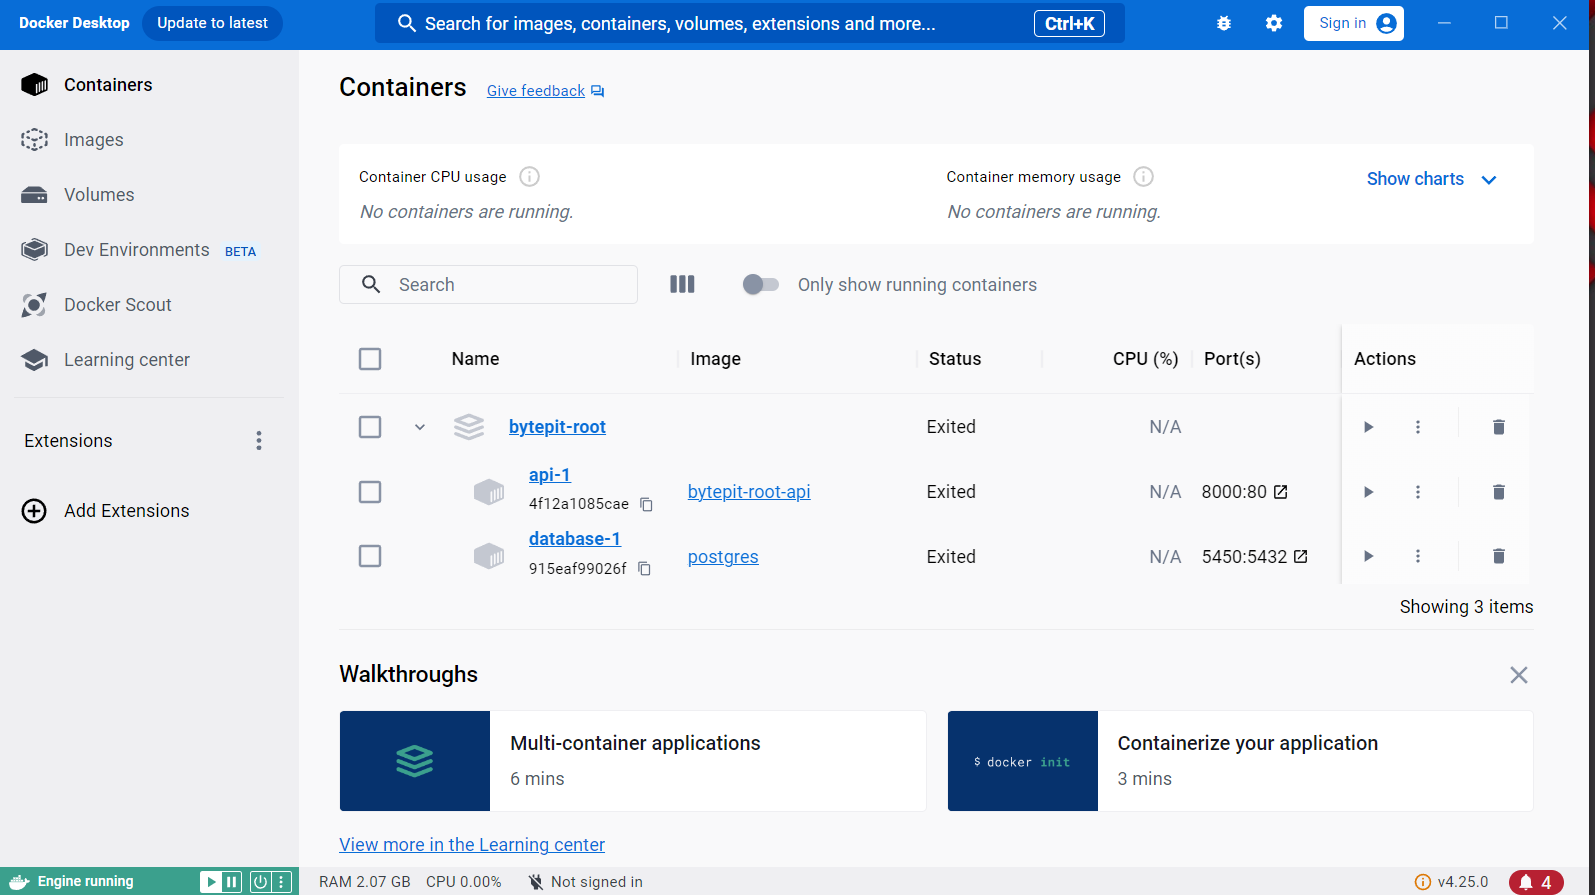
\includegraphics[scale=0.45]{slike/docker_desktop.PNG} 
					\centering
					\caption{Aplikacija Docker Desktop sa kreiranim containerima}
					\label{fig:docker_desktop}
				\end{figure}
				\noindent Pri prvom pokretanju unutar baze neće biti kreirane potrebne tablice, ali ih možemo kreirati uz pomoć datoteke \textbf{ddl.sql} koja se nalazi unutar direktorija \textit{bytepit-root}. Unutar aplikacije Docker Desktop možemo kliknuti na opcije od baze (tri uspravne točkice ispod zaglavlja Actions), te odabrati opciju \textbf{Open in terminal} uz pomoć koje možemo upisati naredbe za kreaciju tablica unutar baze. Unutar terminala odabiremo opciju \textbf{Exec} te u njoj napišemo naredbu: \textbf{psql -U postgres -d db}\\
				\eject
				\noindent Tada možemo pisati naredbe za našu bazu u SQL-u unutar terminala. Sljedeća naredba koju unosimo je cijela \textbf{ddl.sql} datoteka uz pomoć koje se kreiraju tablice. Nakon toga su backend i baza podataka uspješno postavljeni i spremni za korištenje. Kao provjeru za ispravno kreiranje tablica možemo napisati query poput ovoga:\\
				\textbf{SELECT * FROM problems;}, u slučaju ispravnog postavljanja ispisuje se tablica \textit{problems}.\\
				\begin{figure}[H]
					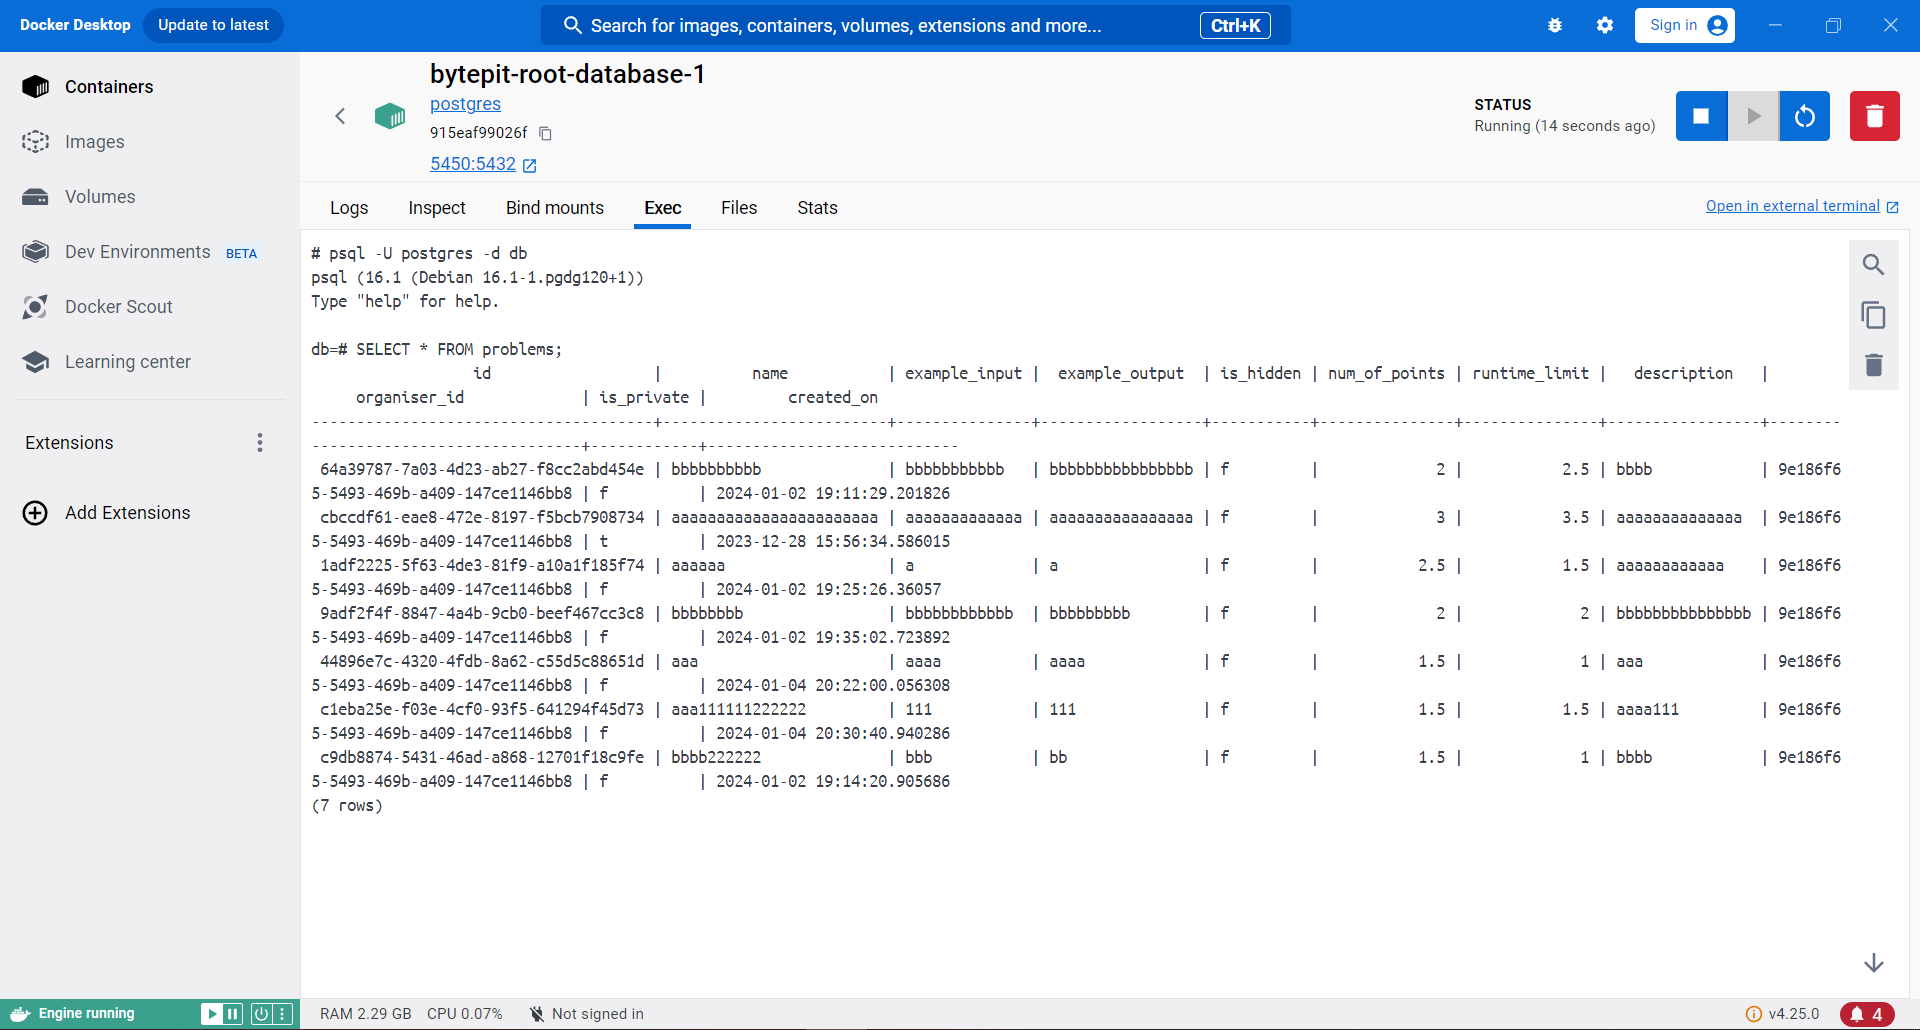
\includegraphics[scale=0.4]{slike/postgres.PNG} 
					\centering
					\caption{Ispravno ispunjena baza i provjera}
					\label{fig:docker_desktop_postgres}
				\end{figure}
				\noindent Za zaustavljanje Docker container-a koristimo naredbu: \textbf{docker-compose down}\\
				
			\eject
			
			\noindent\textbf{Pokretanje frontend-a}\\
			
			\noindent Unutar terminala se navigiramo do direktorija \textit{bytepit-ui} te pokrećemo naredbu: \textbf{npm install}\\
			Pomoću te naredbe se pokreće instalacija Vite-a i ostalih dependency-a koji su potrebni za pokretanje frontend-a. Za instalaciju je potrebno nekoliko minuta.\\
			\noindent Nakon instalacije pokrećemo naredbu: \textbf{npm run dev} koja pokreće frontend.
			\begin{figure}[H]
				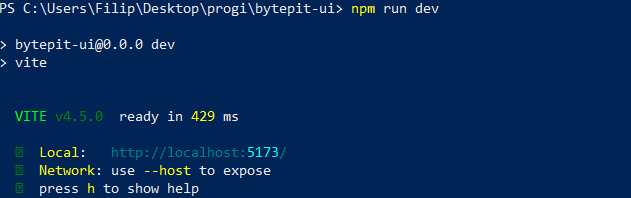
\includegraphics[scale=0.9]{slike/vite.PNG} 
				\centering
				\caption{Terminal nakon uspješno izvedene funkcije za pokretanje}
				\label{fig:vite}
			\end{figure}
			\noindent Tada možemo otvoriti web-preglednik i upisati \textbf{http://localhost:5173/} i početi koristiti aplikaciju.\\
			\begin{figure}[H]
				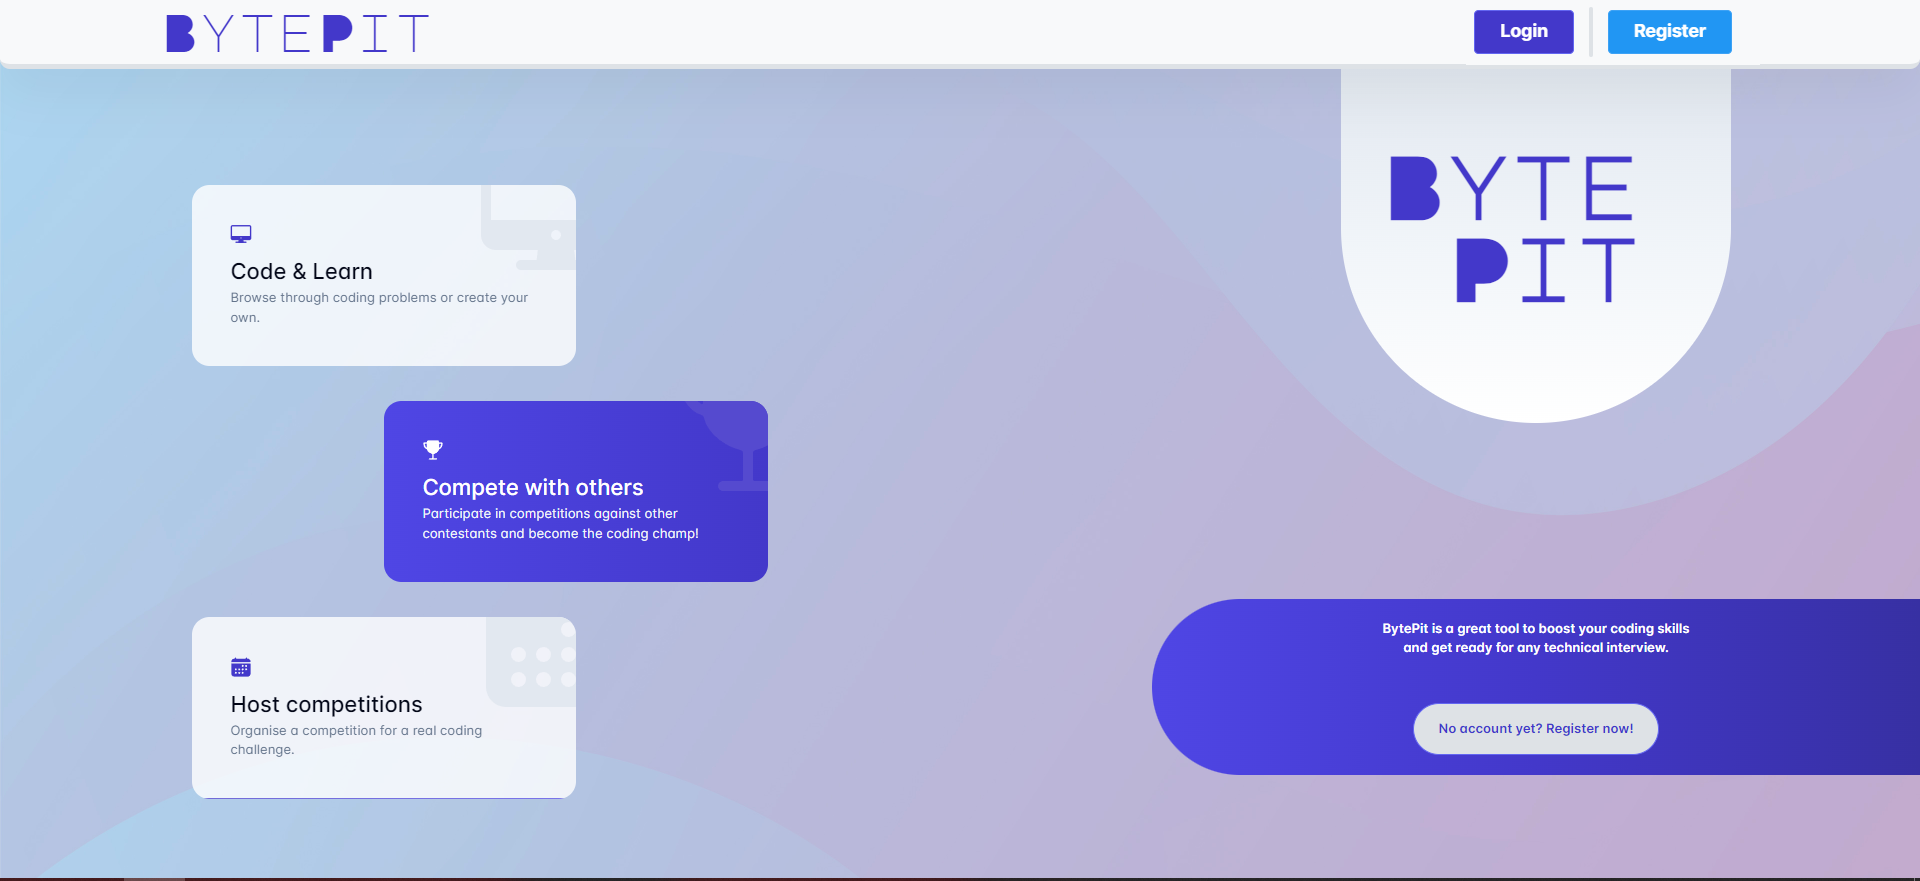
\includegraphics[scale=0.4]{slike/bytepit.PNG} 
				\centering
				\caption{Pokrenuta aplikacija}
				\label{fig:bytepit}
			\end{figure}
			Za zaustavljanje koristimo naredbu: \textbf{npm run stop}\\
			